\chapter{Un poco sobre sistemas Unix}
El software <<\emph{Image Reduction and Analysis Facility}>>, simplemente llamado IRAF, está diseñado para la reducción de imágenes astronómicas. Sin embargo, está disponible exclusivamente para sistemas operativos basados en Unix, tales como GNU/Linux y macOS. Por ello, en esta clase abordaremos los comandos básicos de los sistemas Unix, dándole especial énfasis a GNU/Linux.

\section{Introducción a la línea de comandos}
La línea de comandos, cuyo nombre es \emph{shell}, es una interfaz que proporciona un acceso total a los archivos y procesos de una computadora. Se trata de un programa que toma comandos del teclado escritos por el usuario y luego los pasa al sistema operativo para que los ejecute. Para acceder al shell, se debe usar un emulador de terminal (<<terminal>>, de aquí en adelante) en GNU/Linux o sistemas Unix. En la mayoría de distribuciones de GNU/Linux, la terminal se abre usando la combinación de teclas <<\mintbold{bash}{Ctrl+Alt+T}>>, o alternativamente buscándola en el menú de aplicaciones.

\subsection{Usando la terminal}
Una vez que lances una terminal, deberías ver algo similar a lo siguiente:
\begin{bash}
astronomer@PC:~ $ 
\end{bash}

Los caracteres antes de el símbolo \url{@}, que en este caso dicen <<\texttt{astronomer}>>, representan el nombre de usuario. Lo que aparece después del símbolo \url{@}, representa el nombre de la computadora y en este caso es <<\texttt{PC}>>. Antes de continuar, debes tener en cuenta que el shell es un lenguaje de programación que se ejecuta desde la terminal. Por lo tanto, como cualquier otro lenguaje de programación requiere de comandos, instrucciones de entrada, produce salidas, utiliza caracteres especiales, permite la declaración de variables, etc, como veremos más adelante. El símbolo de dolar (\$) es conocido como el \emph{prompt} de la terminal y nos indica que el shell está listo para recibir comandos. Todos los comandos que escriben después del símbolo \$. 

\subsubsection{El árbol de directorios}
Para poder navegar por el sistema de archivos dentro de un sistema Unix, primero debes entender cómo está estructurada la ubicación de cada directorio (carpeta) dentro de la computadora. A todo el conjunto de carpetas se le conoce como el <<árbol de directorios>>. En los sistemas Unix, la parte superior del árbol de directorios se llama <<directorio raíz>> o simplemente <<root>>. El directorio root está representado con el símbolo <<\texttt{/}>> (una diagonal) y a partir de ahí se despliegan todos los demás directorios, tales como \texttt{bin, dev, home, usr}, entre otros. Dentro de cada uno de esos directorios se despliegan incluso más directorios y así sucesivamente. Como ejemplo particular, dentro del directorio <<\texttt{home}>> se encuentras los usuarios del sistema. En nuestro caso, el usuario es <<\texttt{astronomer}>> y dentro de ese directorio hay otros, llamados <<\texttt{Desktop}>>, <<\texttt{Documents}>>, etc. Puedes visualizar esto con ayuda de la Figura \ref{fig:unix-tree}.

\begin{figure}[htb]
    \centering
    %\includegraphics[width=0.5\linewidth]{}

    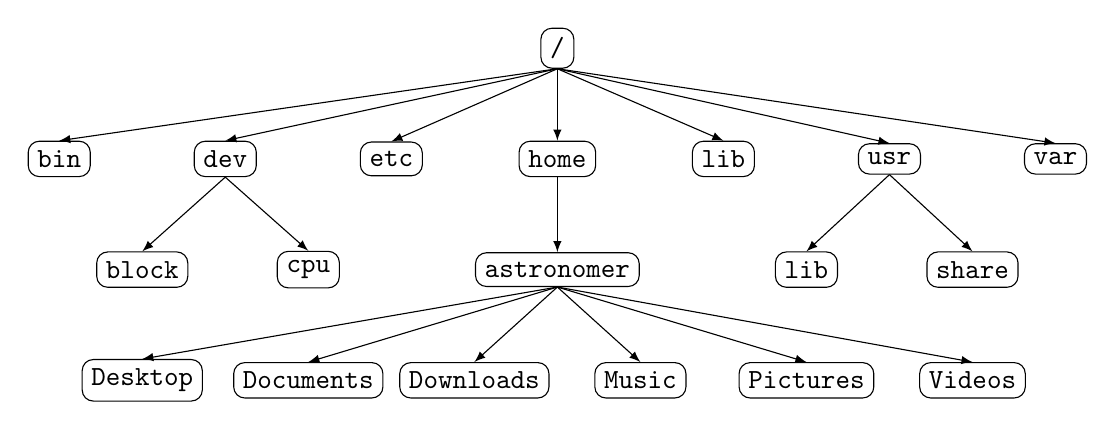
\begin{tikzpicture}[
      grow=down, % Crecimiento del árbol hacia abajo
      edge from parent/.style={draw,-latex},
      sibling distance=6em, % Distancia entre nodos hermanos
      level distance=4em, % Distancia entre niveles
      every node/.style={draw, rectangle, align=center, font=\ttfamily, rounded corners}, % Añade rectángulos y ajusta el estilo
      edge from parent path={(\tikzparentnode.south) -- (\tikzchildnode.north)} % Conecta los nodos desde el centro inferior
      ]
    
      \node {/} % Nodo raíz
        child { node {bin} }
        child { node {dev} 
            child { node {block} }
            child { node {cpu} }
        }
        child { node {etc} }
        child { node {home}
            child { node {astronomer}
                child { node {Desktop} }
                child { node {Documents} }
                child { node {Downloads} }
                child { node {Music} }
                child { node {Pictures} }
                child { node {Videos} }
            }
        }
        child { node {lib} }
        %child { node {tmp} }
        child { node {usr} 
            %child { node {bin} }
            child { node {lib} }
            child { node {share} }
        }
        child { node {var} };
        
    \end{tikzpicture}

    \caption{Diagrama del arbol de directorios en sistemas Unix}
    \label{fig:unix-tree}
\end{figure}

Es posible acceder desde la terminal a cualquiera de los directorios del sistema especificando su <<ruta>>. Las rutas pueden ser absolutas o relativas. En términos generales, las rutas son absolutas si comienzan en la parte superior del árbol de directorios del sistema de archivos, es decir, desde el directorio root. Por lo tanto, las rutas absolutas empiezan con el símbolo \texttt{/}. Tomando como guía la Figura \ref{fig:unix-tree}, la ruta absoluta a la carpeta <<\texttt{Documents}>> es: \mintbold{shell}{/home/astronomer/Documents}.

Las rutas relativas, por el contrario, inician a partir de tu <<directorio actual de trabajo>>, el cual está denotado por un punto (.), mientras que el directorio inmediatamente superior se denota con dos puntos (..). En otras palabras, las rutas relativas inician con un punto o con dos. 

\subsubsection{Imprimir directorio actual con el comando pwd}
Para saber en qué directorio te encuentras actualmente, debes usar el comando <<\mintbold{shell}{pwd}>> (proveniente del inglés \textbf{p}rint \textbf{w}orking \textbf{d}irectory), que mostrará la ruta absoluta a tu directorio actual:

\begin{bash}
astronomer@PC:~ $ pwd
/home/astronomer
\end{bash}

Por defecto, la terminal se abre en el <<directorio personal>>, que para nuestro caso es \mintbold{shell}{/home/astronomer/}. Tomando nuevamente como ejemplo la carpeta <<\texttt{Documents}>>, la ruta relativa hacia esa carpeta desde el directorio personal es simplemente \mintbold{shell}{./Documents}. Por otro lado, la ruta relativa hacia el directorio <<\texttt{home}>> desde el directorio personal es \mintbold{shell}{../}. Nota cómo en el ejemplo anterios, al ejecutar el comando \mintbold{shell}{pwd} se muestra el resultado y aparece nuevamente el prompt esperando nuevas instrucciones.

La ruta absoluta del directorio personal tiene un atajo denotado con una virgulilla (\mintinline{shell}{~}). Como habrás notado, al abrir la terminal aparecen los caracteres <<\mintbold{shell}{astronomer@PC}>> seguidos de dos puntos (:) y el símbolo \mintinline{shell}{~}. A la derecha de los dos puntos se muestra el directorio actual de trabajo. Esto confirma que por defecto, la terminal se abre en el directorio personal.  

\subsubsection{Listar elementos con el comando ls}
Ahora que sabemos en qué directorio nos encontramos dentro de todo el sistema de archivos, veamos qué hay dentro de nuestro directorio de trabajo. Para eso, utilizamos el comando <<\mintbold{shell}{ls}>> (del inglés \emph{list}), que imprimirá la lista de todos los archivos y subdirectorios dentro de nuestro directorio actual:
\begin{bash}
astronomer@PC:~ $ ls
Desktop    Downloads  Pictures  Templates
Documents  Music      Public    Videos
\end{bash}

El comando \mintbold{shell}{ls} dio como resultado la lista de los archivos dentro de la carpeta personal. Uno de esos archivos es una carpeta llamada <<\texttt{Documents}>>. Para ver qué hay dentro de la carpeta <<\texttt{Documents}>>, aplicamos el comando \mintbold{shell}{ls Documents/}, como en el siguiente ejemplo:

\begin{bash}
astronomer@PC:~ $ ls Documents/
Clases-CCD  Datos-CCD  Notebooks-CCD 
\end{bash}

\subsubsection{Cambiar de directorios con el comando cd}
El comando \mintbold{shell}{ls} únicamente nos permite visualizar lo que hay dentro de cada directorio de nuestro interés, pero para navegar dentro de los directorios debemos usar el comando <<\mintbold{shell}{cd}>> (que proviene del inglés \textbf{c}hange \textbf{d}irectory). Para desplazarnos a la carpeta <<\texttt{Documents}>> desde el directorio personal, usamos \mintbold{shell}{cd Documents} o \mintbold{shell}{cd ./Documents}, que son equivalentes:

\begin{bash}
astronomer@PC:~ $ cd Documents
astronomer@PC:~/Documents $
\end{bash}

El comando anterior no produjo ninguna salida, pero cambió nuestro directorio de trabajo. Puedes confirmarlo porque luego de ejecutarlo, los caracteres que aparecen después de los dos puntos (:), cambiaron de <<\mintinline{shell}{~}>> a <<\mintinline{shell}{~/Documents}>>. Si ahora aplicamos el comando \mintinline{shell}{pwd}, nos mostrará el siguiente resultado:

\begin{bash}
astronomer@PC:~/Documents $ pwd
/home/astronomer/Documents 
\end{bash}

El directorio personal se encuentra en el directorio inmediatamente superior del directorio de documentos (ver Figura \ref{fig:unix-tree}). Por lo tanto, la ruta relativa al directorio personal desde el directorio de documentos es \mintbold{shell}{..} y más aún, dentro del directorio personal se encuentra la carpeta <<\texttt{Downloads}>>. De modo que la ruta relativa hacia la carpeta <<\texttt{Downloads}>> desde la carpeta <<\texttt{Documents}>> es \mintbold{shell}{../Downloads}. En otras palabras, podemos acceder a la carpeta <<\texttt{Downloads}>> usando el comando \mintinline{shell}{cd} desde la carpeta <<\texttt{Documents}>> de la siguiente manera:

\begin{bash}
astronomer@PC:~/Documents $ cd ../Downloads
astronomer@PC:~/Downloads $
\end{bash}

Por supuesto que lo anterior pudo haberse logrado de igual manera si se hubiese usado la ruta absoluta, ya sea \mintinline{shell}{/home/astronomer/Downloads} o simplemente \mintinline{shell}{~/Downloads}. Volvamos por ejemplo a la carpeta de Documentos usando su ruta completa:
\begin{bash}
astronomer@PC:~/Downloads $ cd ~/Documents 
astronomer@PC:~/Documents $
\end{bash}

\subsubsection{Crear nuevos directorios con el comando mkdir}
Como hemos visto antes, dentro del directorio \texttt{Documents} hay otros tres directorios llamados \texttt{Clases-CCD,  Datos-CCD} y \texttt{Notebooks-CCD}. Es posible crear nuevos directorios desde la terminal usando el comando <<\mintbold{shell}{mkdir}>> (que proviene del inglés \textbf{m}a\textbf{k}e \textbf{dir}ectory) seguido del nombre de la carpeta que queremos crear. El nombre de la carpeta puede contener guiones (\mintinline{shell}{-}), guiones bajos (\mintinline{shell}{_}) pero no espacios. Si colocamos espacios, \mintinline{shell}{mkdir} creará una carpeta por cada palabra separada por espacios. Para entenderlo mejor, aplica el siguiente comando en la terminal:

\begin{bash}
astronomer@PC:~/Documents $ mkdir New-folder New folder
astronomer@PC:~/Documents $ 
\end{bash}

Lo anterior no produjo ninguna salida. Pero puedes verificar que se crearon unas cuentas carpetas en tu directorio actual:
\begin{bash}
astronomer@PC:~/Documents $ ls
Clases-Datos-CCD  folder  New-folder
Datos-CCD         New     Notebooks-Datos-CCD 
\end{bash}

Como puedes ver, se creo una carpeta llamada <<\mintinline{shell}{New-folder}>>, otra llamada <<\mintinline{shell}{New}>> y una última llamada <<\mintinline{shell}{folder}>>. 

\subsubsection{Crear archivos con el comando touch}
Ahora podemos acceder a la carpeta llamada <<\texttt{New-folder}>> usando \mintinline{shell}{cd New-folder/} y crear unos cuantos archivos. Para eso, necesitamos usar el comando \mintbold{shell}{touch}, seguido del nombre del archivo. Al igual que con mkdir, podemos crear varios archivos al mismo tiempo si los separamos con espacios. Primero ingresamos a la carpeta \texttt{New-folder}:
\begin{bash}
astronomer@PC:~/Documents $ cd New-folder
astronomer@PC:~/Documents/New-folder $ 
\end{bash}

Ahora usamos el comando \mintinline{shell}{touch} dentro de ese directorio:

\begin{bash}
astronomer@PC:~/Documents/New-folder $ touch archivo1.txt archivo2.txt archivo3.pdf archivo4.pdf
astronomer@PC:~/Documents/New-folder $ 
\end{bash}

Lo anterior tampoco produjo ninguna salida, pero podemos verificar que los archivos se crearon. Para eso, usamos el comando \mintinline{shell}{ls}:

\begin{bash}
astronomer@PC:~/Documents/New-folder $ ls
archivo1.txt archivo2.txt archivo3.pdf archivo4.pdf 
\end{bash}

\subsubsection{Crear archivos con el comando ls}
También podemos crear archivos de texto usando el comando \mintinline{shell}{ls}, aunque la sintaxis es diferente. Por ejemplo, supongamos que queremos crear un archivo de texto que contenga el nombre de todos los archivos en nuestro directorio actual. Para lograrlo, usamos la siguiente instrucción:

\begin{bash}
astronomer@PC:~/Documents/New-folder $ ls * > lista_archivos
astronomer@PC:~/Documents/New-folder $
\end{bash}

El símbolo \mintinline{shell}{*} en el comando anterior significa <<todos los archivos del directorio actual de trabajo>>. Mientras que el símbolo \mintinline{shell}{>} significa <<redirigir>> o <<enviar>>. Por supuesto <<\mintinline{shell}{lista_archivos}>> es el nombre del archivo que queremos crear. Como solo escribimos el nombre del archivo, sin ninguna ruta, éste se creará en el mismo directorio donde estamos trabajando. En resumen, el comando anterior puede interpretarse de la siguiente manera: <<lista todos los elementos del directorio actual de trabajo y envíalos a un archivo llamado <<\mintinline{shell}{lista_archivos}>> en este mismo directorio>>. Para verificar que realmente se creó, usamos el comando \mintinline{shell}{ls}:

\begin{bash}
astronomer@PC:~/Documents/New-folder $ ls
archivo1.txt archivo2.txt archivo3.pdf archivo4.pdf lista_archivos
\end{bash}

Observa cómo no fue necesario que especificáramos la extensión del archivo de texto. Es decir, no se necesitó llamar al archivo \mintinline{shell}{lista_archivos.txt}, \mintinline{shell}{lista_archivos.dat} o alguna otra extensión. Si no se brinda ninguna extensión al momento de crear un archivo, el shell asume que se trata de un archivo de texto.

\subsubsection{Visualizar archivos de texto con gedit}
Para visualizar el contenido de \mintinline{shell}{lista_archivos}, puedes usar cualquier editor de texto. Es muy probable que por defecto tengas instalado el editor llamado <<\mintinline{shell}{gedit}>>. Al ejecutar el siguiente comando, debería abrirse el programa \texttt{gedit} con el contenido del archivo \mintinline{shell}{lista_archivos}:

\begin{bash}
astronomer@PC:~/Documents/New-folder $ gedit lista_archivos
\end{bash}

Deberías ver algo similar a esto en la ventana que se abrió:
\begin{bash}
archivo1.txt
archivo2.txt
archivo3.pdf
archivo4.pdf
\end{bash}

Supongamos que estamos interesados en listar únicamente los archivos con extensión \texttt{.pdf} dentro de nuestro directorio. Para eso modificamos un poco nuestra instrucción de la siguiente manera:

\begin{bash}
astronomer@PC:~/Documents/New-folder $ ls *.pdf > lista_pdf
astronomer@PC:~/Documents/New-folder $
\end{bash}

La instrucción anterior puede interpretarse de la siguiente manera: <<Lista todos los elementos del directorio actual de trabajo, cuyos nombres terminen con los caracteres <<\texttt{.pdf}>> y envíalos a un archivo llamado <<\mintinline{shell}{lista_pdf}>> en este mismo directorio>>. 

Ahora utiliza nuevamente un editor de texto, que puede ser \mintinline{shell}{gedit} para verificar el contenido del archivo llamado \mintinline{shell}{lista_pdf}. El contenido de dicho archivo de texto debería ser el siguiente:

\begin{bash}
archivo3.pdf
archivo4.pdf
\end{bash}

Finalmente, para eliminar archivos desde la terminal se utiliza el comando \mintbold{shell}{rm} (que proviene del inglés \textbf{r}e\textbf{m}ove), seguido del nombre del archivo que deseamos eliminar. Al igual que \mintinline{shell}{mkdir} y \mintinline{shell}{touch}, el comando \mintinline{shell}{rm} acepta varios argumentos separados por espacio. Para eliminar los archivos que terminan con la extensión \texttt{.txt} podemos hacerlo uno por uno:

\begin{bash}
astronomer@PC:~/Documents/New-folder $ rm archivo1.txt archivo2.txt
astronomer@PC:~/Documents/New-folder $
\end{bash}

Verificamos que se eliminaron los archivos:

\begin{bash}
astronomer@PC:~/Documents/New-folder $ ls
archivo3.pdf  archivo4.pdf  lista_archivos  lista_pdf
astronomer@PC:~/Documents/New-folder $
\end{bash}

también pudimos utilizar el símbolo \mintinline{shell}{*} para eliminar todos los archivos con extensión \texttt{.txt} de la misma manera que lo usamos con \mintinline{shell}{ls}. Lo aplicaremos para eliminar los archivos con extensión \texttt{.pdf}:

\begin{bash}
astronomer@PC:~/Documents/New-folder $ rm *.pdf
astronomer@PC:~/Documents/New-folder $
\end{bash}
Verificamos que realmente se eliminaron:

\begin{bash}
astronomer@PC:~/Documents/New-folder $ ls 
lista_archivos  lista_pdf
astronomer@PC:~/Documents/New-folder $
\end{bash}

Todos los archivos que creamos eran únicamente ilustrativos. Realmente no los necesitamos ni tampoco a las carpetas que creamos. Regresemos a la carpeta de Documentos:

\begin{bash}
astronomer@PC:~/Documents/New-folder $ cd ..
astronomer@PC:~/Documents $
\end{bash}

Para eliminar carpetas usamos el mismo comando \mintinline{shell}{rm}. Sin embargo, si lo intentas obtendrás un error:

\begin{bash}
astronomer@PC:~/Documents $ rm New-folder/
rm: cannot remove 'New-folder/': Is a directory 
\end{bash}

Para eliminar carpetas necesitamos una instrucción adicional que acompañe al comando \mintinline{shell}{rm}. Estas instrucciones adicionales son llamadas <<banderas>> o <<\emph{flags}>> en inglés. La bandera que necesitamos usar es <<\mintbold{shell}{-r}>>, que le indica al comando \mintinline{shell}{rm} que elimine archivos de manera recursiva:

\begin{bash}
astronomer@PC:~/Documents $ rm -r New-folder
astronomer@PC:~/Documents $ 
\end{bash}
Verificamos que la carpeta se eliminó:
\begin{bash}
astronomer@PC:~/Documents $ ls
Clases-Datos-CCD  Datos-CCD  folder  New  Notebooks-Datos-CCD
astronomer@PC:~/Documents $
\end{bash}

Ahora podemos eliminar las otras dos carpetas que creamos. Recuerda que se llaman <<\texttt{New}>> y <<\texttt{folder}>>. Para eso volvemos a usar el comando \mintinline{shell}{rm} con la bandera \texttt{-r}:

\begin{bash}
astronomer@PC:~/Documents $ rm -r New folder
astronomer@PC:~/Documents $
\end{bash}

Estos son los comandos básicos que se utilizaran para analizar datos usando IRAF. Ahora que ya los conoces, estás listo para instalar IRAF y utilizarlo.

\subsection{Ejercicios}
Estos ejercicios están pensados para que adquieras un mayor entendimiento sobre la navegación en los directorios de sistemas Unix usando la terminal. Serán de utilidad antes de pasar a utilizar Pyraf en la siguiente clase.

Abre una nueva terminal y realiza lo siguiente:
\begin{enumerate}
    \item Dirígete al directorio root usando \mintinline{shell}{cd /}
    \item Desde el directorio root dirígete a tu carpeta personal.
    \item Ejecuta el siguiente comando: 
    \begin{bash}
    cd ..
    \end{bash}

    \item Ahora escribe el siguiente comando y antes de presionar la tecla Enter, presiona la tecla \texttt{Tab}:

    \begin{bash}
    cd ../
    \end{bash}
    Lo anterior te muestra todas las opciones disponibles a las que puedes desplazarte. Elige cualquiera.

    \item Ejecuta el comando \mintinline{shell}{cd} sin ningún argumento:
    \begin{bash}
    cd
    \end{bash}
    Esto te llevará a tu carpeta personal. Dirígete a tu carpeta de descargas usando una ruta relativa.

    \item En tu carpeta personal, usa \texttt{mkdir} para crear una nueva carpeta con el nombre que quieras. Además dentro de esa carpeta crea unas cuantas carpetas más. Utiliza \texttt{touch} para crear archivos vaciós dentro de las carpetas. Utiliza \texttt{ls} para inspeccionar tu trabajo. Ahora utiliza un solo comando para eliminar la carpeta entera.

    \item Utiliza \texttt{ls} para crear un archivo de texto que contenga el nombre de todos los archivos dentro de tu carpeta personal.

    \item Inspecciona el archivo que acabas de crear usando algún editor de texto desde la terminal.

    \item Ahora elimina desde la terminal el archivo de texto que recién creaste.
\end{enumerate}
